\section{\xxx Overview} \label{sec:overview}

Figure 2 shows \xxx's architecture. It contains two main components: 
the Serviceguard and the \smrsystem \smr system.

The \smrsystem component interposes on \tapsend on receiving a network packet 
and runs a RDMA-based consensus process on this request. Besides, this component 
maintains a packet queue to capture outgoing packets by interposing on 
\taprecv and invokes the output checking protocol periodically. 

The Serviceguard component monitors the overall health of the configured applications. 
It sends the application heartbeat to the \smrsystem component in the physical 
host. The Serviceguard uses the application heartbeat as the communication 
medium to convey the status of the application to \smrsystem. If \smrsystem does not 
receive the heartbeat from a particular application within a specified interval, 
the protocol starts leader election and fails over that application to another physical 
host. In addition, the Serviceguard is responsible for checkpoint and restore. 

\begin{figure}[t]
% \vspace{.20in}
\centering
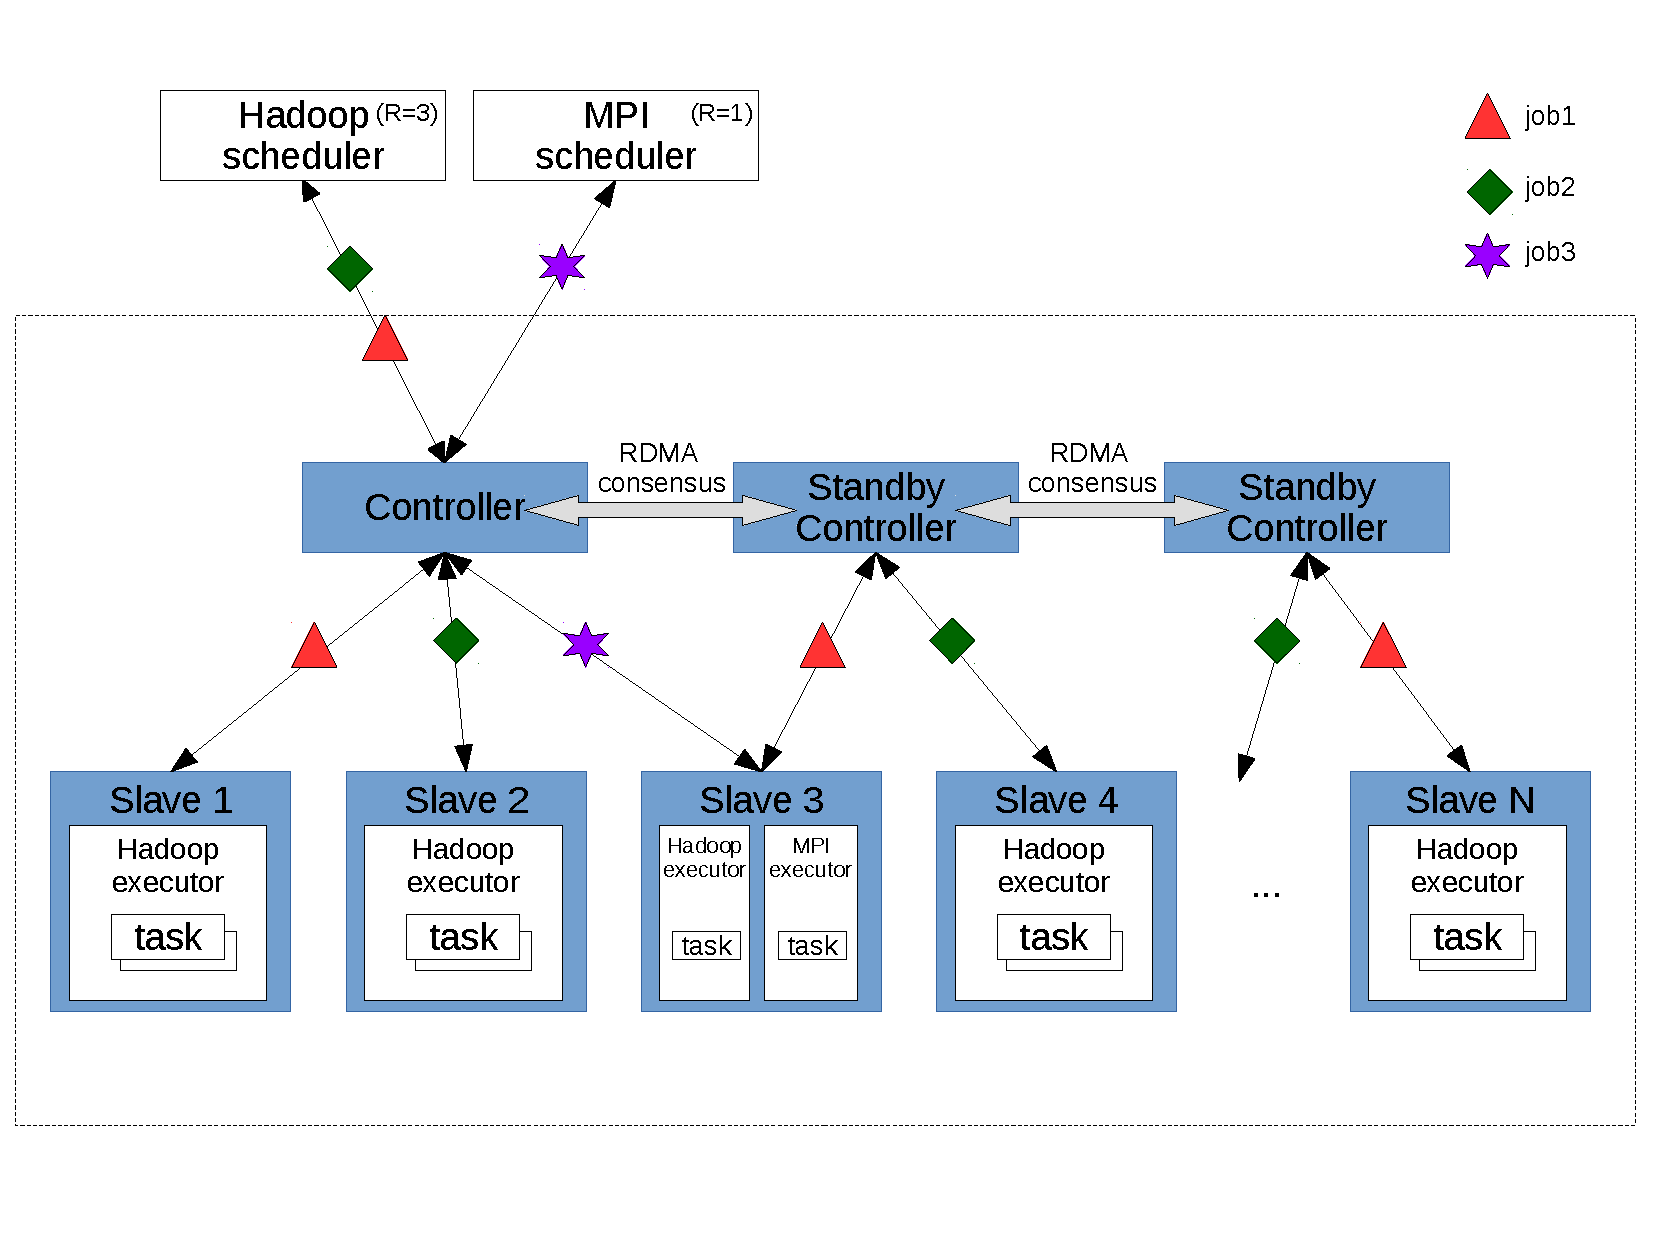
\includegraphics[width=.47\textwidth]{figures/arch}
\vspace{-.2in}
\caption{{\em Proposed architecture in KVM virtualized environment.} Key components are shaded (and
in blue).} \label{fig:arc}
\vspace{.05in}
\end{figure}
